\FloatBarrier
\subsubsection{Injection system}\label{sec:injection}
%\emph{Author(s): P. Wessels, E. Genin and S. Hild \\}

\etbox{h}{hbox:IO_requirements}{Laser beams required at the input of the main interferometers}
{\begin{table}[H]
\centering
\color{\contentcolor}
\begin{tabular}{c|c|c}
\hline
\hline
 & ET-HF &ET-LF\\
\hline
Wavelength &1064\,nm  & 1550\,nm\\
Beam shape & Laguerre Gauss 3,3   & TEM$_{00}$  \\
Optical power in front of  PRM & 500\,W& 3\,W\\
\hline
\hline
\end{tabular}
\end{table}
}

\FloatBarrier
\paragraph{Pre-stabilized laser}

At the development time of second generation GWDs, Neodymium doped Yttrium Aluminium garnet (Nd:YAG) was the best choice as the gain material for 100~W class lasers. However, in the last years, particularly thin disc lasers based on Ytterbium doped crystals have been undergoing a rapid development. The pure power scaling of these systems into the multi-kW range was mainly driven either by material processing or defense applications \cite{Deile2009,Kalisky2010}, which do neither require single-frequency nor fundamental mode output. Nevertheless, good progress has also been achieved in the power scaling of high beam quality laser systems. In particular, near fundamental mode operation with more than 200~W of output power and up to 98~W of single-frequency output power has been demonstrated \cite{Giesen2007}. Further possible advantages are that the 940~nm pump diodes used for e.g.\ Yb:YAG have potentially longer lifetimes than their 808~nm Nd:YAG counterparts and that the lower quantum defect of Yb:YAG causes less thermal effects. However, Yb:YAG is a quasi-3-level system and thus its main disadvantage is that it is more sensitive to increased temperatures within the gain medium.

In order to produce lasers with power levels of several 100~W and to amplify these systems into the kW region, different design concepts are proposed. The main concerns are the thermal management in the gain material and to reduce beam aberrations. In particular, Nd:YAG suffers from a significantly higher quantum defect compared to Yb:YAG making the thermal management even more important. One way to reduce the thermal effects is to use a zig-zag beam path to average over the thermal gradient in the laser crystal. Edge-pumped slab geometries can be combined with conduction-cooling techniques, which avoid vibrations introduced by cooling fluids in conventional layouts. However, one of the main challenges in using slabs is to avoid parasitic oscillations within the high gain regions.

Problems caused by depolarisation and by defocusing can be addressed in different ways. In principle, an efficient birefringence compensation can be implemented~\cite{Lue1996}. However, better than compensating effects is to reduce these. For this, there are in principle two different options. Firstly, \citet{Koechner1971} and \citet{Soms1980} have shown that the amount of depolarisation depends on the Nd:YAG crystal orientation. Therefore, crystal orientations other than the standard [111]-cut could be an option to reduce the depolarisation intrinsically. \citet{Shoji2002} suggested the use of [110]-cut crystals in combination with small beam size in the high pumping regime to reduce depolarisation. In recent experiments~\cite{Puncken2010}, the [100]-, [110]- and [111]-crystal orientations were compared in a single pass configuration in the pump power regime relevant for 2nd generation GWD. Although these results are very promising in terms of intrinsic reduction of depolarisation effects, they also show that the non-symmetrical shape of the thermal lens in unconventionally cut crystals might limit the achievable beam quality in laser oscillators.

The second option is to reduce the thermal gradients which cause these stress-induced birefringence effects. As shown in the work by \citet{Wilhelm2009,Wilhelm2010}, the maximum peak temperature of an end-pumped laser rod or slab can be reduced by the use of laser rods composed of several segments with different doping concentrations. 
The quantum defect and therefore the overall heat load in a Nd:YAG laser media can be reduced by more than 30\% by changing the pump wavelength from 807~nm to 885~nm (see e.g.~\cite{Lavi2000,Frede2006}).
Core doped rods can be used (see e.g.~\cite{Kracht2006}) to achieve an easier and more stable fundamental mode operation.
In these rods only the inner core is doped and the outer core is used as a waveguide for the pump light comparable to a double clad fibre as described by \citet{Bedoe1993}. This concept is similar to mode selective pumping as the gain is only present in the doped inner core of the rod. However, it has the advantage that no high brightness pump source is required.

Optical fibre amplifiers have a large potential to offer single-frequency output at higher efficiencies and lower cost than solid-state amplifiers at similar power levels (see for example the overview paper by~\citet{Limpert2007}). Until several years ago, diode-pumped fibre amplifiers were limited to power levels of several Watts. This was both due to the unavailability of high brightness pump diodes as well as due to nonlinear effects in the fibre such as stimulated Raman scattering and stimulated Brillouin scattering (SBS).
The invention of large mode-area (LMA) fibres and of photonic crystal fibres (PCF) has enabled output powers of single-mode fibre lasers to exceed 1~kW while retaining excellent efficiencies (see for example~\citet{Jeong2004}). The large effective core diameter of these fibres decreases the average intensity of the light at the laser wavelength in the fibre and thereby increases the threshold of nonlinear processes. The large inner cladding of the double-clad LMA fibres allows high power multi-mode pumps to be coupled into the fibre. Despite the large diameter of the active core, a clean single-mode output can be obtained by suppressing the higher order transverse modes by bending losses. A typical PCF geometry and a representative beam profile of such a fibre is shown in Fig.~\ref{fig:pcf_geometry}. The limiting factor for \emph{narrow-linewidth} high-power fibre lasers for the use in GWDs is the onset of SBS.

\begin{figure*}[h]
\begin{center}
  \begin{tabular}[c]{c}
    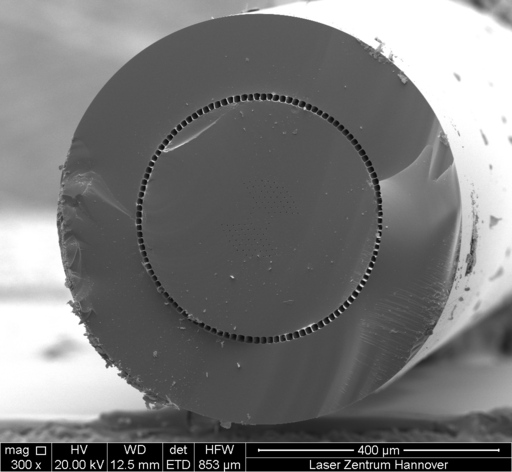
\includegraphics[width=0.4\textwidth]{./Sec_Optics/sem_picture_pcf}
  \end{tabular}
  \hspace*{1cm}
  \begin{tabular}[c]{c}
    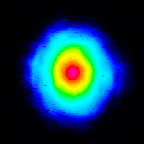
\includegraphics[width=0.25\textwidth]{./Sec_Optics/beamprofile_pcf}
  \end{tabular}
  \caption{Typical geometry of a large-core photonic crystal fibre (left) and typical beam profile (right).}
  \label{fig:pcf_geometry}
\end{center}
\end{figure*}

A state-of-the art single-frequency fibre amplifier system with 150~W of output power with a good output beam profile (92\% in TEM$_{00}$) is described in~\cite{Hildebrandt2006}. With this system an optical-to-optical efficiency of 78\% with respect to incident pump power was achieved with a good polarisation ratio of about 100/1. Recently, the output power of single-frequency, PCF-based, Ytterbium-doped fibre amplifiers has been scaled to more than 400~W of output power \cite{Robin2010}.

A different approach to realize LMA fibres with excellent output beam quality and simultaneously larger mode areas are multifilament-core (MFC) fibres with core regions consisting of many small doped filaments.  In contrast to conventional multi-core design, the multifilament core fibres aim for strong coupling between smaller filaments resulting in the propagation of only one supermode by adequately choosing the diameter and spacing of the filaments. In the last years, MFC fibres with active and also with passive filaments were demonstrated, which enabled transversely single-mode output with a nearly Gaussian-shaped intensity mode profile~\cite{Canat2008,Vogel2009}. The main advantage of this new fibre type is the low effective core numerical aperture which can be achieved without the need for flattening the refractive index profile as it is crucial for PCFs. This is of particular importance for large index core materials like Erbium-Ytterbium codoped fibres for which this design approach allows for a precise reduction and control of the effective core index. Important properties of the MFC fibres, e.g.\ the low bending losses, can be explained using an equivalent step index based on the theory of the fundamental space filling mode~\cite{Canat2010}. Recently, it has been demonstrated that a TEM$_{00}$ mode content of more than 95\% can be achieved with such an actively doped fibre~\cite{Kuhn2010}. In Fig.~\ref{fig:mfc_mode}, both the calculated as well as the measured mode profile of an Erbium-Ytterbium codoped MFC fibre with 37 filaments is shown.

\begin{figure*}[h]
\begin{center}
  \begin{tabular}[c]{c}
    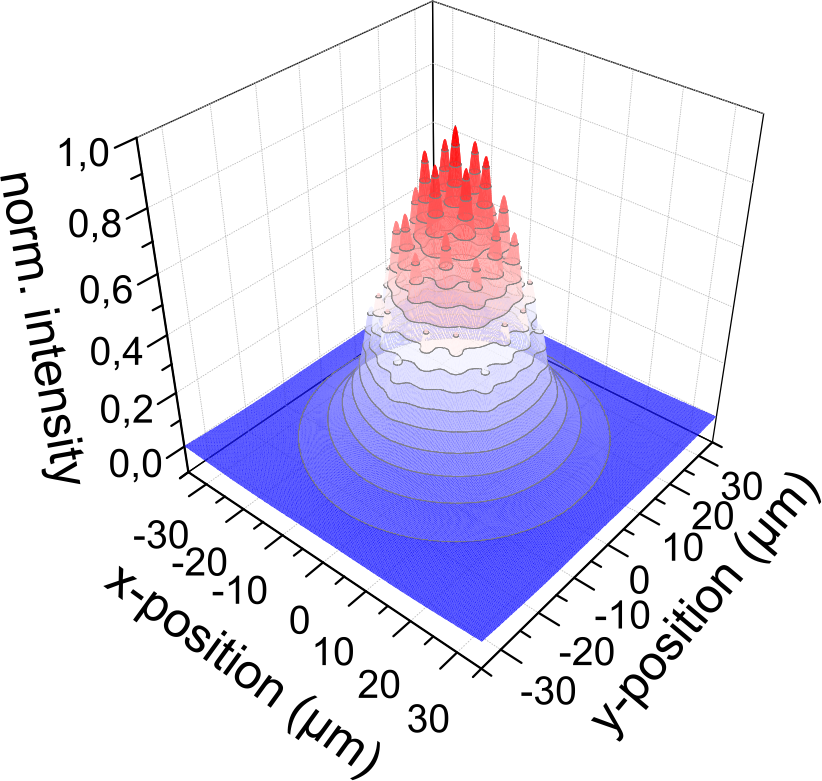
\includegraphics[width=0.45\textwidth]{./Sec_Optics/mfc_mode_calc.png}
  \end{tabular}
  \hspace*{1cm}
  \begin{tabular}[c]{c}
    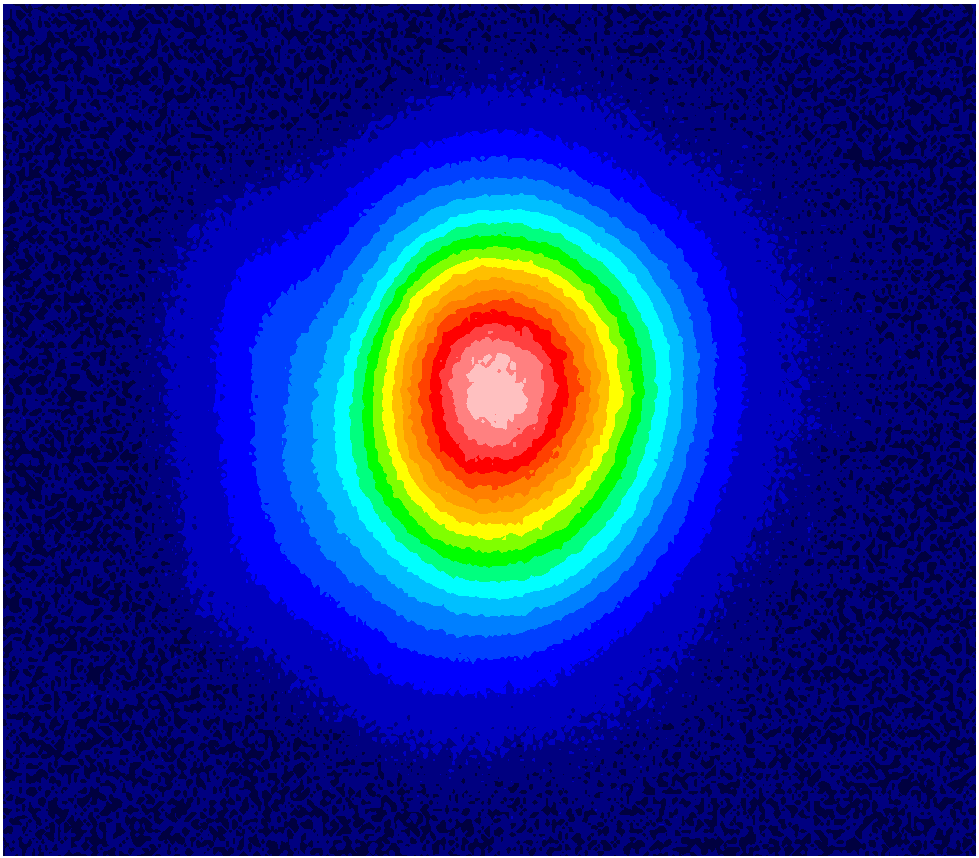
\includegraphics[width=0.25\textwidth]{./Sec_Optics/mfc_mode}
  \end{tabular}
  \caption{Calculated mode profile for an Er-Yb multifilament-core fibre with 37 filaments (left) and measured mode profile (right) with a fundamental Gaussian mode content of more than 95\%.}
  \label{fig:mfc_mode}
\end{center}
\end{figure*}

Novel ideas to increase the SBS threshold are under investigation. A promising concept is to shift the Brillouin frequency along the fibre to lower the effective Brillouin gain for each frequency component. This could be achieved by temperature or strain gradients, or by varying doping concentrations along the fibre.
Furthermore, fibres with specially designed transverse refractive index profiles are being developed to minimize the overlap of the optical and the acoustical fibre modes, also resulting in an effective reduction of the Brillouin gain.

Besides the power scaling aspect, the reliability and noise performance of high power fibre lasers need to be further analyzed and possibly improved to meet the requirements of third generation gravitational wave detectors. Especially thermal effects and contamination at the air-glass interface have to be considered. The main problem is the large light intensity at these interfaces which could be reduced by use of an undoped beam expansion section at the fibre ends or by all-fibre solutions for the pump-light coupling. One big advantage of fibre lasers is that they are compact and simple compared to the complex solid-state laser systems. Furthermore, modern splice techniques allow to produce monolithic all-fibre systems including the master oscillator, the high power stage and possibly even a mode-cleaning fibre, if required.

Erbium-doped fibre lasers emit around 1.56~$\mu$m where the absorption in silicon is small compared to the silica substrates currently used at 1~$\mu$m wavelength. For an efficient design with low nonlinear effects in single frequency operation, the Erbium-doped fibre should have high pump absorption and should be as short as possible. Unfortunately, the pump absorption cross sections of Erbium are about a factor of 10 lower than those of Ytterbium. In addition, quenching effects also limit the sensible doping concentrations to about a factor of 10 below that of Ytterbium. These combined factors result in about two orders of magnitude lower pump absorption of Erbium doped fibres, if similar fibre geometries as used with Ytterbium doped fibres are assumed. In order to avoid excessive fibre lengths, which is necessary to circumvent the onset of SBS, either the signal-core to pump-core ratio has to be adapted or the amplifier even has to be pumped into the single-mode signal core. For these reasons, pump sources with very high brightness or even single-mode beam quality are needed. This becomes even more obvious if the typically achieved optical-to-optical efficiencies of about 25\%--30\% (50\% for 1480~nm pumping) are compared with the typical value of ${}>70\%$ for Ytterbium. Recently, a single-mode output power of 81~W at 1480~nm was demonstrated with a Raman fibre laser~\cite{Nicholson2010} which can be used as a pump source for single-mode Er based systems. However, commercially available single-mode Raman fibre laser modules are currently limited to an output power of 10--20~W.

In order to overcome these limitations, Yb codoping of Er-doped fibres and pumping at 980 nm can be used. This allows high pump absorption but also implicates a second gain band at the Yb wavelength around 1~$\mu$m. This second gain bands limits the achievable output power due to the onset of massive amplified spontaneous emission (ASE) which finally leads to pulsing instabilities of the amplifier system. The highest single-frequency output power of 151~W achieved with this concept was accompanied by more than 70~W of ASE at 1~$\mu$m~\cite{Jeong2005}. Nevertheless, in recent experiments a new scheme was demonstrated by which the 1~$\mu$m oscillation in an Er-Yb codoped fibre amplifier could be effectively suppressed~\cite{Kuhn2009}.

Concerning the direct generation or the amplification of spatial beam profiles other than the fundamental (fibre) mode, only very limited experimental results have been published. A good overview is given in the review article by~\citet{Ramachandran2008}. For the generation of specific higher order modes, the laser light is first coupled into the fundamental LP$_{01}$ mode of a single-mode fibre. Then, an in-fibre long-period Bragg grating converts the LP$_{01}$ into the desired LP$_{0m}$ mode. This process can be very efficient with peak efficiencies of more then 99\%. The usage of higher order modes in the optical fibres has several advantages compared to the fundamental mode. Firstly, the effective mode area is significantly enlarged and hence the threshold for SBS is increased. Furthermore, the higher order modes are less sensitive to mode distortions due to fibre bending or refractive index profile imperfections due to the fibre fabrication process. Recently, fibre amplifiers have been demonstrated employing this technique for the first time in an active fibre with several Watts of output power~\cite{Nicholson2010a,Nicholson2010b}. However, all higher order LP$_{0m}$ modes used have a central high intensity peak in common which is undesirable for the use in GWD~\cite{Vinet2009}. Thus, some research on the generation of axisymmetric fibre modes with an intensity minimum in the centre as well as on the amplification of these modes will have to be carried out. Most probably, this will also involve some special design of active fibres in which the active dopant distribution favors the amplification of the mode of interest.

\etbox{r}{rbox:lasers}{Lasers for ET}
{
While the step from first to second generation gravitational wave detectors required
to scale the laser systems up by about a factor of 20, the step from second generation
to ET will only require a much smaller scaling factor of about 4 for ET-HF.
Research programs on ET lasers are already under way and no fundamental limits are known
which are expected to prevent the realisation of the high power laser for ET-HF.
The laser power
required for ET-LF is with only about 5\,W very small and currently already available.
}

\FloatBarrier
\paragraph{Injection optics}


%\textbf{Overview and General requirements}

The Input Optics system (IO) of ET takes care of the optics downstream of the lasers. The whole system must deliver a beam with the required power, geometrical shape, frequency and angular stability at the Interferometer input.




%
%%\bigskip
%\begin{table}[h]
%\centering
%%\begin{center}
%\begin{tabular}{l l l}
%\hline \hline
%{\bf Requirement} & {\bf Value at 1064 nm} & {\bf Value at 1550 nm}\\
%\hline
%Laser power available at the interferometer input & 500\,W   & 3\,W\\
%\hline
%Intensity noise & TBD & TBD\\
%\hline
%Beam jitter noise (misalignment mode amplitude) & TBD & TBD\\
%\hline
%IMC cavities throughput & $>80\%$ on LG$_{33}$ & $>80\%$ on TEM$_{00}$\\
%\hline
%IO overall throughput & $>50\%$ on LG$_{33}$ & $>50\%$ on TEM$_{00}$\\
%\hline \hline
%\end{tabular}
%%\end{center}
%\caption{Requirements for the ET Input Optics (IO) system \label{table:ET-IO}}
%\end{table}
%%\bigskip

Electro-Optic Modulators (EOM) should provide the needed RF phase or amplitude modulations
(to sense longitudinal and angular degrees of freedom; see section \ref{sec:control}). Two in-vacuum suspended input mode cleaners (IMC)
in series will be used to geometrically clean the beam and reduce its amplitude fluctuations as well as geometrical fluctuations. The
resonant IMC could also serve in the loop of laser frequency stabilization. After the IMC an intensity stabilization
section will provide the signal for stabilizing the laser's relative intensity noise (RIN)
and reach the requirements. An in-vacuum Faraday
isolator (FI) will prevent interaction of the interferometer reflected light with the IMC and laser system. Finally, a mode matching telescope will be used to
provide a beam with the correct size and wave front curvature  for matching it into the interferometer.
It is planned to use super-polished optics for ET-HF and ET-LF in order to lower as much as possible potential diffused
light noise.
Moreover the beam pointing noise created in components in free-space propagation (mirrors, lenses, EOM, FI,
etc.) can be dominated by acoustic, seismic and thermal noise. Particular effort will be given to isolate
the optics from seismic noise. Furthermore, several sensors used in the control loops will be placed on
suspended benches inside the vacuum vessel of ET.

\paragraph{Input Mode Cleaner}

The laser light must be frequency- and spatially stabilized before it can be used in the interferometer.
 The input mode cleaner  provides active frequency stabilization through feedback to the laser and passive
frequency noise suppression above its cavity pole frequency. %, and passive spatial stabilization at all frequencies.
The input mode cleaner also reduces higher order modal content of the laser light, suppressing beam jitter by a
factor depending of the cavity finesse.

%\subsection{IMC for ET-HF}

The baseline configuration of the IMC for ET-HF is to use two 20-meter
long IMC cavities placed in series (as done in GEO interferometer).
Due to the high laser power that will be stored in the IMC cavity,
radiation pressure effects and absorption in the  IMC cavity
input and output mirrors will be the main limiting effects. The radiation pressure effects
 will depend on the cavity
finesse chosen. In Advanced Virgo, with about 60\,kW power stored in this
cavity it has been shown that the radiation pressure effect on the angular
degrees of freedom is manageable by using mirrors of at least 3\,kg weight~\cite{RPnote}.
This means that this effect could be overcome by increasing the IMC
mirror weight or reducing the finesse if possible. For
the lock acquisition of the cavity it is likely that we need to lock the
cavity at a lower power and go to full power once the
cavity is locked~\cite{RPnote}. Radiation pressure noise (linked to
power fluctuation in the cavity) could also be responsible
for frequency noise since it can affect the length of the IMC cavity
and the angular control of the IMC end mirror if the beam
 is not well centered on this mirror. In the linear regime, it has been
 shown that radiation pressure noise was not an issue for
initial Virgo sensitivity~\cite{RPnoise} and Advanced Virgo~\cite{INJPDS}.
%Specifications on this noise will have to be given for ET.
Concerning input and output mirrors absorption, in order to
avoid beam distortion induced by photothermal effects, a low-absorption
fused silica grade with good homogeneity should be
chosen as mirror substrate and coating absorption lower than 1
ppm is mandatory~\cite{IMCcharac}.
In order to cope with higher order Laguerre-Gauss modes,
the resonant mode cleaner should be made with an even number
of mirrors as explained in~\cite{barsu,chelkow}.
Cavity parameters (finesse, round-trip losses and cavity pole)
will have to be defined according to the beam jitter, amplitude
and frequency noise requirements at the interferometer input.

%\subsection{IMC for ET-LF}

There are two main differences between the input mode cleaners for ET-HF and ET-LF:
First of all the optical power in the ET-LF IMC will be orders of magnitude
lower than in the ET-HF IMC and therefore we expect to encounter fewer potential issues
related to radiation pressure and thermal effects in the ET-LF IMC.
 Secondly the laser wavelength of the ET-LF IMC will
be 1550\,nm, which will allow us to strongly profit from
synergies with the telecommunication sector. Therefore, we believe the realisation
of the ET-LF IMC to be less challenging than the IMC for the ET high frequency interferometers.

%Due to the fact that a number of things have been developed in the 1550\,nm
%wavelength range for telecommunications, we will
%try to use as much as possible of the already existing components for the
%IMC of the ET-LF interferometers.
%For ET-LF, we have 2 possibilities to make a spatial filtering of the laser beam:
%\begin{itemize}
%\item use a resonant mode-cleaner as done in ET-HF
%\item use an optical fibre.
%\end{itemize}
%Some R\&D activity is needed on this subject to see if the optical fibre
%is able to fulfill ET requirements. In any case, a resonant cavity will
%probably be needed at least to stabilize the laser frequency.
%The baseline solution remains to use two 20-meter long triangular cavities
%in series where we have more experience and know that this kind of
%suspended cavity will fulfill our requirements.
%As for ET-HF, IMC parameters should be defined according to beam
%stability, laser frequency and amplitude stability required at the interferometer input port.

\paragraph{Faraday isolator}

In order to avoid unwanted cross-coupling, light back-reflected by the interferometer should
be picked up before being coupled back in the IMC cavities. The solution adopted in first
and second generations of gravitational wave detectors is to install a Faraday isolator in
vacuum on the beam path between the interferometer and the input mode cleaner cavity.

\emph{Faraday isolator for ET-HF:}
Faraday isolator designs have evolved to cope with the increase of power between first
and second generation detectors. A R\&D program put in place at the European Gravitational
Observatory in collaboration with the Institute of Applied Physics (Nyzhni Novgorod Russia) has
developed a Faraday isolator with reinforced magnetic field and using a thermal depolarization
 compensation technique~\cite{Khazanov_compensation}. This isolator uses Terbium Gallium
 Garnett (TGG) as magneto-optic material and the design has been optimized for thermal
 depolarization, thermal lensing and Verdet constant change compensation~\cite{HPIOfinal}.
 This device is able to achieve very good isolation performances (${}>38$\,dB) in vacuum from
 low power up to 250\,W laser power~\cite{genin}.
We could use this experience and the same kind of design and scale it up to get the expected
performances of the Faraday isolator in the 1\,kW power range.
For ET-HF we could expect that the in-vacuum Faraday isolator should have the following characteristics:
\begin{itemize}
\item withstand high average power (1\,kW) on long periods;
\item an optical isolation higher than 30\,dB at full power;
\item residual thermal lensing resulting in a focal length higher than 100\,m;
\item provide good transmission (at least 95\%)
\end{itemize}

\emph{Faraday isolator for ET-LF:}
In the telecom wavelength range, TGG cannot be used due to its higher absorption at 1550\,nm. Fortunately,
in the field of telecommunications a lot of possible materials are available that can
 be used for Faraday isolators~\cite{mavalvala}. The main aspect that needs to be checked
 for ET-LF is ultra-high vacuum compatibility of a 1550\,nm Faraday isolator.


 % In any case, as for the high power Faraday isolator needed for ET-HF, the development of vacuum compatible Faraday isolator for 1550\,nm wavelength requires to build up a test facility and collaborative work with laboratories or companies having experience with free space Faraday isolator adapted to telecom wavelength. The relatively low power used in the configuration will probably simplify the design of such an isolator with respect to the ET-HF high power Faraday isolator.

\paragraph{RF-Electro optical modulation system}
\nopagebreak

In ET radio-frequency (RF) modulation of the laser beam will be used in the control of the interferometer, both for longitudinal and angular controls.

\emph{RF modulation system for ET-HF:}
The main difference between the Electro Optical Modulation (EOM) system to be used in ET-HF respect to first and
second generation detectors is the laser power that the EOM system will have to withstand (up to 1\,kW for ET-HF).
Thermal effects become more significant~\cite{Mansell} and the choice of an appropriate material (electro-optic  crystal)
 becomes crucial to limit the consequences of these thermal effects on the EOM performance. Indeed, it is
 important to select the right material not only to limit wavefront aberrations but also to reduce local temperature fluctuations
 of the material. This heating can induce slow variations of the modulation index and therefore disturb the interferometer control.
The ET requirements  for the electro optical modulation system (oscillator phase noise, modulation index and modulation
index noise) will have to be defined in the technical design, as many of these parameters will affect the driving electronics and signal generator choice.

\emph{RF modulation system for ET-LF:}
The experience of telecommunication field will be used extensively in the RF-modulation system of ET-LF. It is likely that integrated fibered optical components will be used to modulate the laser light.

\paragraph{Other high power compatible components}
\nopagebreak

The selection and development of high power compatible components suitable for ET-HF is essential. Experience acquired during the Advance Virgo highpower input optics R\&D program should be a good starting point in the selection of waveplates, polarizers and for the design of high power low diffusing beam dumps~\cite{HPIOfinal,genin}.

%\paragraph{R\&D work needed for ET}
%\nopagebreak
%
%Laser and injection optics of ET can benefit of the many years of R\&D already performed within the  Advanced LIGO, Advanced Virgo and GEO-HF
% projects in investigating high power compliant components such as electro-optical modulators and Faraday isolators.
%
%For ET it is necessary to carry out the following two R\&D programs: the first one will be focussed on ET-HF components
%that have to be compliant with high power laser and the LG$_{33}$ mode. The second one should concern ET-LF and the
%development and selection of IO components (Faraday isolator, EOM, mirrors, waveplates and polarizers). Laser beam
% cleaning through a fiber has also to be studied for this configuration.
% %Collaboration with experienced people (laboratories
% %or companies) is essential in the success of these two R\&D programs.

